\subsection{Sprachsynthese}

Dieses Kapitel beschreibt die Integration der Sprachsynthese in das Praxisrufsystem.
Der Fokus liegt dabei auf den Abläufen zum Empfangen von Benachrichtigungen und dem Abrufen von Sprachdaten.
Die Integration von notwendigen Schnittstellen im Mobile Client wird im Kapitel 5.2 beschrieben.

\subsubsection{Konfiguration}

Nach Use Case U03\footnote{Siehe Kapitel 3} muss der Praxismitarbeitende alle Sprachbenachrichtigungen stummschalten können.
Dazu wird der Mobile Client um eine Settings Ansicht erweitert.
Auf dieser Ansicht, kann der Benutzer auswählen, ob Benachrichtigungen vorgelesen werden sollen.
Ist die Option deaktiviert, werden Benachrichtigungen nie vorgelesen.

Benachrichtigungen für Praxisruf können über das Admin UI konfiguriert werden.
Es kann pro Benachrichtigung Titel, Inhalt, Anzeigetext für Benachrichtigungsbuttons und eine Beschreibung erfasst werden.
Diese Konfiguration wird über die Entität NotificationType verwaltet.
Neu soll auch konfiguriert werden können, ob eine Benachrichtigung für die Sprachsynthese relevant ist.
Dazu wird die Entität NotificationType um ein boolean Flag mit dem Namen isTextToSpeech erweitert.
Dieses Flag wird beim Versenden einer Benachrichtigung mitgesendet und kann vom Empfänger überprüft werden.
Insofern Sprachbenachrichtigungen in den Einstellungen aktiviert sind, werden Benachrichtigungen, welche dieses Flag auf TRUE gesetzt haben vorgelesen.

\begin{figure}[h]
    \centering
    \begin{minipage}[b]{0.75\textwidth}
        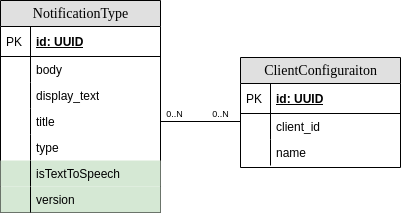
\includegraphics[width=\textwidth]{/home/joshua/FHNW/dev/IP6/IP6_Bachelorarbeit_Bericht_Cloudbasiertes_Praxisrufsystem/src/graphics/diagramms/erd_t2s_v01.drawio}
        \caption{ERD Ausschnitt - Konfiguration Sprachsynthese}
    \end{minipage}
\end{figure}

Neben dem Feld isTextToSpeech, wird die NotificationType Entity um ein weiteres Feld version erweitert.
Dieses Version Feld beinhaltet eine Ganzzahl welche mit jeder Änderung inkrementiert wird.
Das Version Feld wird ebenfalls beim Versenden von Benachrichtigungen mitgesendet und kann auf Client Seite zur Implementierung eines Caches verwendet werden.


\clearpage

\subsubsection{Integration Cloud Service }

Die Anbindung des Sprachsynthese Service erfolg zentral über den Cloudservice.
Dazu wird der Cloudservice um ein Modul Speech erweitert.
Das Speech-Modul soll gleich wie die Module Configuration und Notification keine direkten Abhängigkeiten auf andere Cloud Service Module haben.
Sämtliche notwendige Kommunikation zwischen den Modulen findet über Rest-Schnittstellen statt.
Diese Unabhängigkeit ermöglicht es, das Modul zukünftig aus dem Cloud Service auszubauen und als eigenständigen Micro-Service zu betreiben.

\lstinputlisting[caption=SpeechSynthesisService.java,language=java,label={lst:SpeechSynthesisService.java}]{listings/SpeechSynthesisService.java}

Für dieses Projekt wird AWS Polly verwendet.
Dementsprechend wird das SprachSyntheseService Interface für AWS Polly implementiert.
AWS Polly bietet einen Java SDK, welcher die Anbindung ermöglicht.
Dieser SDK bietet alle Klassen die für die Anbindung an AWS Polly nötig sind.
Da im Cloudservice Spring Boot verwendet wird, können die für die Verbindung nötigen Klassen mit einer Spring Config erstellt werden
und dann über Dependency Injection im AwsPollySpeechSynthesis Service verwendet werden.

\lstinputlisting[caption=AwsConfiguration.java,language=java,label={lst:AwsConfiguration.java}]{listings/AwsConfiguration.java}

In der Implementation des Services kann nun über den injezierten AmazonPollyClient eine Abfrage an den Speech Synthesis Service gesendet werden.

\clearpage

\subsubsection{Schnittstelle Cloud Service}

Das Speech-Modul stellt einen Endpoint zur Verfügung über den die Sprachdaten zu einer Benachrichtigung abgefragt werden können.
Der Endpoint bietet dabei nicht die möglichkeit generische Daten in Sprachdaten zu verwandeln.
Stattdessen erlaubt er es Sprachdaten für die aktuelste Version von bekannten Benachrichtigungstypen zu beziehen.
Der einzige Parameter für diese Anfragen ist die technische Identifikation des Benachrichtigungstyps (NotificationType) der relevanten Benachrichtigung.
Anhand dieses Identifikators können die Informationen des Benachrichtigugnstyps über die REST-Schnittstelle des Configuration-Modul angefragt werden.
Dadurch können Änderungen an einem Benachrichtigungstyp direkt angewendet werden, ohne dass die Informationen auf dem Mobile Client aktualisiert werden müssen.
Die geladenen Daten können dann verwendet werden um eine Anfrage an den Sprachsynthese Provier zu senden.
Die vom Provider gelieferten Sprachdaten können anschliessend als Resultat an den Client zurügegeben werden.

Der Endpunkt für die Abfrage von Sprachdaten im Cloud Service wird als Spring RestController umgesetzt.
Die Sprachdaten werden dabei als Binärdaten mit Media Type "audio/mp3" im Body der Response zurückgegeben.
Auf Client Seite, kann dieser Endpunkt so als Download angesprechen werden.

\lstinputlisting[caption=SpeechSynthesisController.java,language=java,label={lst:SpeechSynthesisController.java}]{listings/SpeechSynthesisController.java}

Auf Client seite kann dieser Endpunkt nun als Download angesprochen werden.

\subsubsection{Integration Mobile Client }

\lstinputlisting[caption=PraxisrufApi+Speech.swift,language=swift,label={lst:PraxisrufApi+Speech.swift}]{listings/PraxisrufApi+Speech.swift}

Um die Anbindung im Cloudservice vom konkreten Anbieter möglichst unabhängig zu machen, wird die Integration an den Speech Synthese Service über ein Interface abstrahiert.
Soll ein neuer Sprachsyntese Service angebunden werden, muss lediglich dieses Interface für den neuen Service implementiert werden und alles andere kann unberührt bleiben.

\clearpage

\subsection*{Laufzeitsicht}

Benachrichtigungen für welche Sprachsynthese aktiviert ist, sollen beim Empfang automatisch vorgelesen werden.
Dazu müssen die Sprachdaten geladen werden, wenn die Benachrichtigung empfangen werden.
Diese Daten können über den neuen Speech Endpoint des Cloudservices bezogen werden.
Die Informationen die dazu nötig sind, sind als Metadaten in der empfangenen Benachrichtigung vorhanden.

\begin{figure}[h]
    \centering
    \begin{minipage}[b]{0.9\textwidth}
        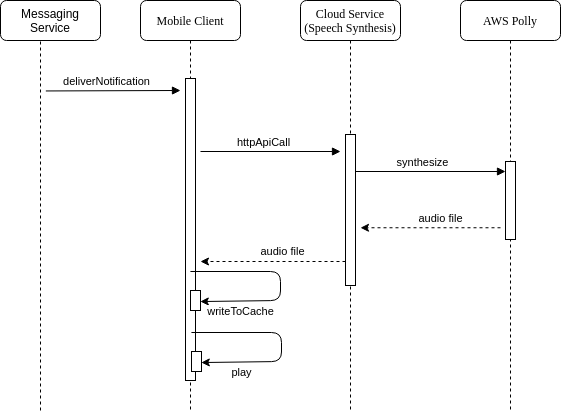
\includegraphics[width=\textwidth]{graphics/diagramms/Sequence_Speech_Synth_V01}
        \caption{Ablauf Benachrichtigung empfangen}
    \end{minipage}
\end{figure}

Wird eine Benachrichtigung empfangen, wird die Benachrichtigung auf dem Client als Push Notifikation angezeigt und an die Inbox übergeben.
Anschliessend prüft der Client ob die Sprachdaten für die Empfangene Benachrichtigung bereits lokal zur Verfügung stehen.
Dies wird gemacht in dem er überprüft ob es im Applikationsverzeichnis bereits eine MP3-Datei für den Empfangenen Benachrichtigungstyp
(NotificationType) in der Version der Empfangenen Benachrichtigung vorhanden ist.
Sind die Daten bereits lokal vorhanden, wird keine Abfrage an den Cloudservice gespielt sondern die lokal vorhandene Sprachdatei abgespielt.
Sind die Daten lokal nicht oder nur in einer anderen Version vorhanden, werden die Daten beim Cloudservice angefragt.
Sobald diese Daten geladen sind, werden sie in einer MP3 Datei mit Id und Version des Benachrichtigungstyps (NotificationType) gespeichert.

\clearpage
